\documentclass{beamer}
\usecolortheme{crane}
\usepackage[utf8]{inputenc}
\usepackage{graphicx}
\usepackage{alltt}
\usepackage{myrules}
\newcommand{\arrowitem}{\item[\mantriangleright]}

\newcommand\singleitem[1]{%
\begin{itemize}
  \item #1
\end{itemize}
}

\author{Benus Becker}
\title[EasyOcaml]{EasyOcaml}
\subtitle{}
\date{28. Januar 2009}
\institute{Universität Freiburg \\ Institut für Informatik \\ Abtg.\ für Programmiersprachen}
\keywords{}
\subject{}

\begin{document}

\frame{\titlepage}

\begin{frame}[fragile]{Ein Beispiel}
  \centerline{\tt let f b x y = x + if b then y ;;}
  \begin{description}
    \item[Objective Caml version 3.11.0]\ \\
      \texttt{\# let f b x y = x + \underline{if b then y} ;;\\
      Error: This expression has type unit but is here used with type int}
    \item[EasyOCaml]\ \\
      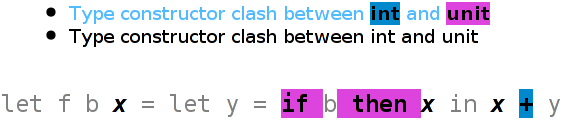
\includegraphics[rotate=90,width=0.75\textwidth]{mightadd}
  \end{description}
\end{frame}

\begin{frame}{Ziele}
  \begin{itemize}
    \item Fehlermeldungen verbessern
      \begin{itemize}
        \item Parser
        \item Typchecker
      \end{itemize}
    \item didaktische Hilfsmittel
      \begin{itemize}
        \item Einschränkungen der Syntax
        \item Bereitstellung von Code
      \end{itemize}
    \item Integration in das existierende OCaml System
      \begin{itemize}
        \item Nutzen der existierenden Codegenerierung
        \item Zugriff auf vorhandene Programmbibliothek
      \end{itemize}
  \end{itemize}
\end{frame}

\begin{frame}{Verwandte Projekte}
  \begin{description}
    \item[Haack \& Wells (2004)]\ \\
      \begin{itemize}
        \item Constraint-basiertes Typchecken von MiniML
        \item minimale, ausreichende Darstellung der Gründe
      \end{itemize}
    \item[Helium]\ \\
      \begin{itemize}
        \item Haskell Compiler ``für Anfänger''
        \item Hinweise zum Lösen der Typfehler
      \end{itemize}
    \item[DrScheme]\ \\
      \begin{itemize}
        \item Standard IDE für Programmierkurse in Scheme
        \item einfacher Debugger
        \item Language Levels und Teach Packs
      \end{itemize}
  \end{description}
\end{frame}

\begin{frame}{Unterstützte Sprache}
  Caml$_{-m}$: Caml ohne Moduldeklarationen
  \begin{description}
    \item[Werte]
      Primitive, Tupel, Listen, Arrays, Varianten, Records, Funktionen, Ausnahmen.
    \item[\emph{Structure items}]
      Typ-, Ausnahmen-, Wertdeklarationen und Expressions.
    \item[\emph{Pattern}]
      Geschachtelt auf alle möglichen Werte.
    \item[Ausdrücke]
      Konstruktoren, Ausnahmebehandlung, Konditionale, Abstraktionen, Typannotationen.
  \end{description}
  \note{Einschränkbar durch Language Levels}
  \note{Alle Teile der stdlib ohne format typbar}
\end{frame}

\begin{frame}{Einbettung in OCaml}
  Ablauf von EasyOCaml
  \begin{itemize}
    \item Kommandozeilenparameter: \texttt{-easy}, \texttt{-easyerrorprinter},
      \texttt{-easylevel}, \texttt{-easyteachpack}
    \item Syntaxanalyse mit Camlp4
    \item Constraintbasierte Typrekonstruktion
    \item Zurückführung in den Compiler bzw.\ die REPL
  \end{itemize}
\end{frame}

\begin{frame}{Typchecker}
  \framesubtitle{Haack \& Wells, 2004}
    \texttt{\# let f b x y = x + \underline{if b then y} ;;\\
   * Type error: Type constructor clash between int and unit.
   Slice: .. + if .. then .. else () ..}
  \begin{itemize}
    \item Ziele
      \begin{itemize}
        \item mehrere Fehler auf einmal berichten
        \item Fehler sind minimal und vollständig\note{definieren}
      \end{itemize}
    \item Haack \& Wells' Typchecker für MiniML
      \begin{enumerate}
        \item Generierung von Constraints
        \item Lösen von Contraints
        \item Aufzählen der Fehler
        \item Minimierung der Fehler
      \end{enumerate}
    \item Gleichzeitig mit Constraintgenerierung: Unbekannte Variablen erkennen
  \end{itemize}
\end{frame}

\begin{frame}{Typchecker}
  \framesubtitle{Erweiterungen für EasyOCaml}
  \begin{itemize}
    \item Syntaktische Kategorien
      \begin{description}
        \item[Deklarationen] $\Delta;\ strit \Downarrow_s \langle \Delta,\ C,\ u\rangle$
        \item[Ausdrücke] $\Delta;\ lexp \Downarrow_e \langle ty,\ C,\ u\rangle$
        \item[Pattern] $\Delta;\ pat \Downarrow_p \langle ty,\ C,\ b\rangle$ 
      \end{description}
    \item Typen: Varianten, Records
\inferrule[Variant] {
  \Delta\onvar(K) = \langle ty_r,\ [ty_{a,1},\ \dots,\ ty_{a,n}]\rangle \\
  \etyjudge \Delta {lexp_i} {ty_i} {C_i} {u_i} \text{ for } i=1,\dots,n \\
  C_0 = \{a \xlongequal l ty_r \} \cup \{ ty_i \xlongequal l ty_{a,i}\ |\ i=1,\dots,n \} \\
  a \fresh
} {
  \etyjudge \Delta {(K\  lexp_1\ \dots\ lexp_n)^l} a {\bigcup_{i=0}^n C_i} {\bigcup_{i=1}^n u_i}
}
    \item Typannotationen $(lexp : ct)$
      \begin{itemize}
        \item $lexp$ und Kontext werden unabhängig getypt
        \item Validität der Annotation wird nachträglich geprüft
          \note{Annotation wird als korrekt angenommen}
      \end{itemize}
  \end{itemize}
  \note{mehr mögliche Fehler}
\end{frame}

\begin{frame}{Fehlerbehandlung}
  Drei Klassen von Fehlern
  \begin{itemize}
    \item Einfach: Erkannt während Constraintgenerierung und -lösen
    \item Schwer: Erkannt während Constraintgenerierung, danach gemeldet
    \item Fatal: Syntaktische Fehler
  \end{itemize}
  Anpassung der Fehlermeldungen
  \begin{itemize}
    \item Internationalisierung der Fehlerbeschreibung
    \item Formatierung für unterschiedliche Ausgaben
  \end{itemize}
\end{frame}

\begin{frame}{Language Levels und Teach Packs}
  Definition und einfache Auslieferung verfügbarer Sprachkonstrukte und
  vordefiniertem Codes
  \begin{description}
    \item[Sprachkonstrukte] Deaktivierung von Optionen für die nicht-terminale Deklaration, Ausdruck, Pattern im Parser
    \item[Vordefinierter Code] \ldots
  \end{description}
\end{frame}

\begin{frame}{Änderungen am Parser}
  EasyOCaml parst mit Camlp4 Parser
  \begin{itemize}
    \item hart kodiertere Beschreibung
    \item Streamparser erlauben nur Zeichenketten als Information
  \end{itemize}
\end{frame}

\begin{frame}{Weiter Entwicklungen}
  \begin{itemize}
    \item[\checkmark] Typchecker für Teilsprache von OCaml
    \item[\checkmark] Internationalisierte und anpassbare Fehlermeldungen
    \item[\checkmark] Hilfsmittel für die Lehre mit OCaml
    \item[\checkmark] Integration in original Compiler und REPL
    \item[\checkmark] Anpassbare Fehlermeldungen für den Parser
    \item[\checkmark] HTML Fehlerausgaben
    \item[\checkmark] Portierung auf OCaml 3.11
    \item Integration in DrOCaml oder Camelia
    \item Heuristiken/Tips zum Lösen von Fehlern
    \item Fehlermeldungen mit mehr Informationen versehen
    \item selbstdokumentierende Language Levels und Teach Packs
    \item ungetypter Interpreter
  \end{itemize}
\end{frame}

\begin{frame}{Fazit}
  \begin{itemize}
  \end{itemize}
  \begin{itemize}
    \item Zweigeteilt: Arbeit am Typchecker -- Integration in OCaml
    \item moderne Forschungsergebnisse (Haack \& Wells) anwenden
    \item OCaml verbessern und open source zu arbeiten
  \end{itemize}
\end{frame}

\begin{frame}{Quellenangaben}
  \bibliographystyle{chicago}
  \clearpage\bibliography{easyocaml}
\end{frame}

\end{document}
